\subsection[定义和性质]{复变函数的积分}
有了复变函数微分的基础,我们现在来讨论积分.复变函数的积分的定义可以同实变函数积分的类比得到.
在复平面上取一个路径$\ell$,起终点为$A(z_0),B(z_n)$,沿着该路径定义了一连续函数$f(z)$,用$n-1$个点$z_1, z_2,\cdot, z_{n-1}$将该路径
$\ell$分成$n$个线段(见图\ref{fig:complex_integral}).函数$f(z)$在线段$z_{k-1}\rightarrow z_{k}$上任意一点$\xi_k$的值乘上线段的长度$\Delta z_k = z_k - z_{k-1}$并求和,即
\begin{equation}
    S_n = \sum_{k=1}^{n} f(\xi_k) (z_{k} - z_{k-1}) .
\end{equation}
\begin{figure}[htbp]
    \centering
    \input{tikz/integral.tex}
    \caption{复变函数积分示意图.光滑曲线$\ell$上取一系列点$z_k$将其分成$n$小段.}
    \label{fig:complex_integral}
\end{figure}
当$n\to \infty$, 求和则转化为积分.当这个和的极限存在且
与$\xi_k$的选取无关时,这个极限称为
函数$f(z)$沿着路径$\ell$的\textbf{路径积分}(Contour integral), 记作
$\int_{\ell} f(z) dz$,即
\begin{equation}
    \int_{\ell} f(z) dz = \lim_{n\to \infty} \sum_{k=1}^{n} f(\xi_k) (z_{k} - z_{k-1}) . 
\end{equation}
其实,我们还可以将该定义用实虚部的方式表达出来,
\begin{align}
    \int_{\ell} f(z) dz  & = \int_{\ell} \left( u(x,y) + \imath v(x,y) \right) (dx + \imath dy) 
    \\
    & = \int_{\ell} \left( u(x,y) dx  -  v(x,y) dy \right) + \imath \int_{\ell}  \left( v(x,y) dx  + u(x,y)dy \right) 
\end{align}
这样一来,复变函数的路径积分就转化成了两个实变函数的线积分.因此,很多实函数线积分的性质可以应用在复变函数路径积分上.

\begin{example}
计算曲线积分
\[
\int_{l} z^{2}\,dz
\]
其中终点为 \(A=(2,i)\)，起点为原点 \(O\)。分别沿路径 (1)——从 \(O\) 到 \(A\) 的直线段；以及路径 (2)——先沿实轴从 \(O\) 到 \(B=(2,0)\)，再从 \(B\) 垂直上升到 \(A\)——计算该积分，并比较结果。
\end{example}
\begin{center}
% 若需要图形，请确保文档导言区加载了 tikz：
% \usepackage{tikz}
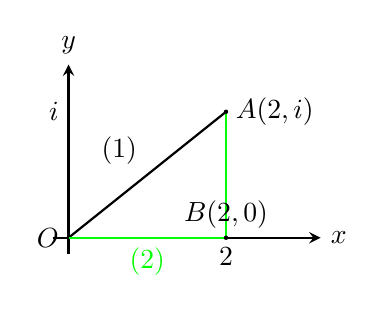
\begin{tikzpicture}[>=stealth,scale=1.0]
    % 坐标轴
    \draw[->,thick] (-0.2,0) -- (3.2,0) node[right] {$x$};
    \draw[->,thick] (0,-0.2) -- (0,2.2) node[above] {$y$};
    \node[left] at (0,0) {$O$};
    % 点 A(2,i) 与 B(2,0)
    \coordinate (A) at (2,1.6); % 这里用比例画出 i 的位置
    \coordinate (B) at (2,0);
    % 路径 (1)
    \draw[thick] (0,0) -- (A) node[midway,above left] {$(1)$};
    % 路径 (2)
    \draw[thick,green] (0,0) -- (B) node[midway,below] {$(2)$}
                      -- (A) node[midway,right] {};
    % 标记点与刻度
    \fill (A) circle (0.8pt) node[right] {$A(2,i)$};
    \fill (B) circle (0.8pt) node[above] {$B(2,0)$};
    \node[below] at (2,0) {$2$};
    \node[left] at (0,1.6) {$i$};
\end{tikzpicture}
\end{center}

\begin{solution}
先写出复函数的形式
\[
z^2 = x^2 - y^2 + i\,2xy.
\]

\textbf{路径 (1)：} 直线段 \(O\to A\)。

参数化取
\[
z(t)=(2+i)t,\qquad 0\le t\le 1,
\]
因此 \(dz=(2+i)\,dt\) 且
\[
z(t)^2=(2+i)^2 t^2=(3+4i)\,t^2.
\]
于是
\[
\int_{(1)} z^2\,dz
=\int_{0}^{1} (3+4i)t^2\,(2+i)\,dt
=(3+4i)(2+i)\int_{0}^{1} t^2\,dt.
\]
计算常数乘积与定积分：
\[
(3+4i)(2+i)=2+11i,\qquad \int_0^1 t^2\,dt=\frac{1}{3},
\]
因此
\[
\boxed{\;\int_{(1)} z^2\,dz=\frac{2}{3}+\frac{11}{3}i\;.}
\]

\bigskip

\textbf{路径 (2)：} 分两段，记为 (2a) 和 (2b)。

(2a) 实轴段 \(O\to B\)，参数化 \(z=x\) (\(0\le x\le 2\))，有 \(dz=dx\)，且 \(z^2=x^2\)。于是
\[
\int_{(2a)} z^2\,dz=\int_{0}^{2} x^2\,dx=\left.\frac{x^3}{3}\right|_{0}^{2}=\frac{8}{3}.
\]

(2b) 垂直段 \(B\to A\)，参数化 \(z=2+i y\) (\(0\le y\le 1\))，有 \(dz=i\,dy\)。计算
\[
z^2=(2+i y)^2=4- y^2 + i\,4y.
\]
因此
\[
\int_{(2b)} z^2\,dz
=\int_{0}^{1} (4- y^2 + i\,4y)\,i\,dy
=\int_{0}^{1}\big(4i - i y^2 -4y\big)\,dy.
\]
对每项积分得
\[
\int_0^1 4i\,dy = 4i,\quad
\int_0^1 (-i y^2)\,dy = -\frac{i}{3},\quad
\int_0^1 (-4y)\,dy = -2.
\]
故
\[
\int_{(2b)} z^2\,dz = -2 + \frac{11}{3}i.
\]

将两段相加得到路径 (2) 的总积分：
\[
\int_{(2)} z^2\,dz
= \frac{8}{3} + \Big(-2 + \frac{11}{3}i\Big)
= \frac{2}{3} + \frac{11}{3}i.
\]

\bigskip

两条路径的结果一致：
\[
\boxed{\;\int_{(1)} z^2\,dz=\int_{(2)} z^2\,dz=\frac{2}{3}+\frac{11}{3}i\;.}
\]
这符合期望，因为 \(f(z)=z^2\) 在全平面解析，因此对同一端点的曲线积分与路径无关（亦可由柯西定理/原函数原理说明：原函数为 \(F(z)=\tfrac{1}{3}z^3\)）。
\end{solution}



